\section{Three Task Result}

We now extend the above idea to three tasks. In this scenario, let our tasks be denoted as $A$, $B$, and $C$. Task $A$ produces output consumed by task $B$, which in turn produces output consumed by task $C$. We want to limit the age of the output of $A$ that is eventually used by $C$.

For this scenario, define $d_{A \to C}$ as the maximum age of the data produced by task $A$ that is used by task $C$. Note that we are not making any assumptions about when a job of task $B$ is executed between jobs of tasks $A$ and $C$. The formalization is similar to the two task scenario:

\begin{equation*}
	\begin{aligned}
		& \text{Given:}
		& & E^{*,*}_A, E^{*,*}_B, E^{*,*}_C, P_C \text{ and } d_{A \to C} \\
		& \text{Find:}
		& & P_A \text{ and } P_B \\
		& \text{That Minimizes:}
		& & U(T) = \sum_i \frac{E_i^{u,max}}{P_i} \\
		& \text{Subject To:}
		& & 
	\end{aligned}
\end{equation*}
\begin{equation*}
	\forall i, r^i_C - f_B^{C_B(r^i_C)} + E^{u,max}_B + r_B^{C_B(r^i_C)} - f_A^{C_A(r_B^{C_B(r^i_C)})} \leq d_{A \to C}
\end{equation*}

\noindent Note that we assume worst case execution and data delay for task $B$. This will produce a more urgent local deadline that will enforce freshness also when this does not occur. More rigorously, let $\delta = E_B^{u,max} - E_B^{l,min}$. Using the max value as we do instead of the least value decreases $d_{B \to C}$ by $\delta$. As can be seen from Lemma~\ref{lem:2TaskResult} this decreases $P_B$ by $\delta / 2$. Viewing task $B$ and $C$ alone as their pair, it is easier to see that the freshness is made of two periods of $B$ for a total decrease of $\delta$. Hence, in the case of minimal execution of task $B$ the execution increases by $\delta$ but this same amount has already been compensated for in the formulation.

The execution of the three tasks is outlined in the figure \ref{fig:3Tasks}.

\begin{figure}[!ht]
	\centering
	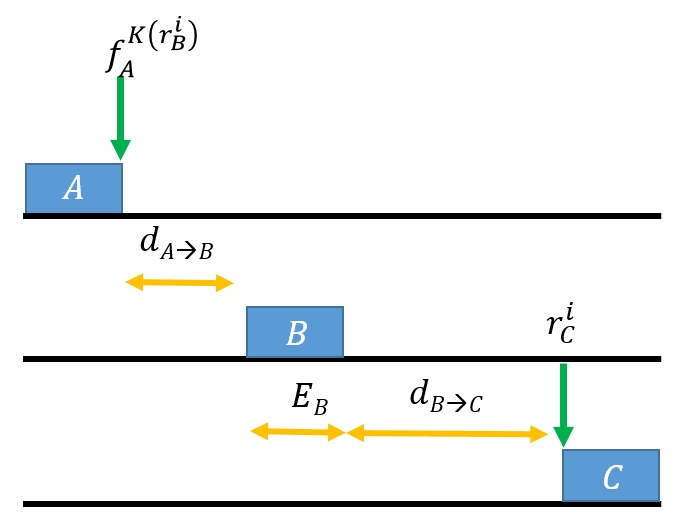
\includegraphics[width=0.3\textwidth]{figures/3TaskMaxStaleness}
	\caption{Maximum Staleness Scenario for Data from Task A.}
	\label{fig:3Tasks}
\end{figure}

Figure~\ref{fig:3Tasks} labels the several intervals in the execution of the three tasks. Note how between tasks $A$ and $B$ and between tasks $B$ and $C$ we've added local freshness constraints. By meeting these two freshness constraints, the freshness of data from task $A$ to task $C$ is ensured. These added constraints will not be present in our final solution but are added here to allow us to introduce Lemma~\ref{lem:2TaskResult} while considering task $B$. These local constraints are used as free variables in our optimization, and once determined we will use our lemma to calculate period assignments that rely only on the end-to-end constraint and task execution times.

From Figure~\ref{fig:3Tasks} we can see that the maximum age of the data from task $A$ used by task $C$, $d_{A \to C}$, is the sum of three values. Concretely,

\begin{center}
	$d_{A \to C} = d_{A \to B} + E^{u,max}_B + d_{B \to C}$
\end{center}

We now use our lemma to extend the two task result to this scenario. Using Lemma \ref{lem:2TaskResult}\ldots

\begin{center}
	$P_A \leq \frac{d_{A \to B} + E^{l,min}_A}{2} \text{ and } P_B \leq \frac{d_{B \to C} + E^{l,min}_B}{2}$
\end{center}

Our lemma uses the BCET for the first task in each pair in order to maximize the possible staleness. For our freshness guarantee, we will use the BCET to be pessimistic with the data age, whereas when calculating utilization we will use the WCET. That is, our solution will ensure freshness even in with best-case execution of the first task, while minimizing the maximum utilization the system could experience.

We simplify the objective by removing constants from the utilization expression and then transform it by substituting from Lemma~\ref{lem:2TaskResult}, using equality since lower periods increase utilization:

\begin{align*}
	U(T) &= \left(\frac{E^{u,max}_A}{P_A} + \frac{E^{u,max}_B}{P_B}\right) &\mbox{Objective}&\\
	&= \left(\frac{E^{u,max}_A}{\frac{d_{A \to B} + E^{l,min}_A}{2}} + \frac{E^{u,max}_B}{\frac{d_{B \to C} + E^{l,min}_B}{2}}\right) &\mbox{Substitution}&\\
	&= \frac{2E^{u,max}_A}{d_{A \to B}+E^{l,min}_A} + \frac{2E^{u,max}_B}{d_{B \to C}+E^{l,min}_B} &\mbox{Simplification}&
\end{align*}

We minimize this objective to arrive at the following solution.

\begin{theorem}
	\label{thm:3TaskResult}
	Given $E^{*,*}_A$, $E^{*,*}_B$, $E^{*,*}_C$, and $P_C$, to minimize utilization while enforcing the freshness bound $d_{A \to C}$, choose
	\begin{align*}
		P_A &= \frac{\sqrt{\frac{E^{u,max}_A}{E^{u,max}_B}}(E^{l,min}_B+d_{A \to C}-E^{u,max}_B+E^{l,min}_A)}{2(1+\sqrt{\frac{E^{u,max}_A}{E^{u,max}_B}})}\\
		P_B &= \frac{\sqrt{\frac{E^{u,max}_A}{E^{u,max}_B}}(E^{l,min}_A+E^{l,min}_B)+d_{A \to C}-E^{u,max}_B+2E^{l,min}_B}{2(1+\sqrt{\frac{E^{u,max}_A}{E^{u,max}_B}})}
	\end{align*}
\end{theorem}

\begin{proof}
	This optimization can be solved using elementary calculus methods. We will use Lagrangian multipliers to optimize the local constraints and then use Lemma~\ref{lem:2TaskResult} to assign periods.
	
	First we set up the Legrangian optimization problem:
	\begin{center}
		$\frac{2E^{u,max}_A}{d_{A \to B}+E^{l,min}_A} + \frac{2E^{u,max}_B}{d_{B \to C}+E^{l,min}_B} + \lambda (d_{A \to C}-d_{A \to B}-E^{u,max}_B-d_{B \to C})$
	\end{center}
	
	We now take partials with respect to our free variables, $d_{A \to B}$ and $d_{B \to C}$, and then set the partials equal to zero to solve for $\lambda$:
	
	%\begin{center}
	%	$\frac{\partial}{\partial d_{A \to B}} = -\frac{2 E^{u,max}_A}{(E^{l,min}_A+d_{A \to B})^2}-\lambda
	%	\text{ and }
	%	\frac{\partial}{\partial d_{B \to C}} = -\frac{2 E^{u,max}_B}{(E^{l,min}_B+d_{B \to C})^2}-\lambda$
	%\end{center}
	
	%We set these equal to zero and solve for our $\lambda$'s \ldots
	\begin{align*}
	-\frac{2 E^{u,max}_A}{(E^{l,min}_A+d_{A \to B})^2}-\lambda &= 0 \to \lambda = -\frac{2 E^{u,max}_A}{(E^{l,min}_A+d_{A \to B})^2}\\
	-\frac{2 E^{u,max}_B}{(E^{l,min}_B+d_{B \to C})^2}-\lambda &= 0 \to \lambda = -\frac{2 E^{u,max}_B}{(E^{l,min}_B+d_{B \to C})^2}
	\end{align*}
	
	With two values of $\lambda$ we can form an equality which we can use with our constraint equation in a system of equations to solve for $d_{A \to B}$ and $d_{B \to C}$. We'll solve for $d_{A \to B}$ first:
	
	%\begin{align*}
	%	-\frac{2 E^{u,max}_A}{(E^{l,min}_A+d_{A \to B})^2} &= -\frac{2 E^{u,max}_B}{(E^{l,min}_B+d_{B \to C})^2}\\
	%	d_{A \to B}+E^{u,max}_B+d_{B \to C} &= d_{A \to C}
	%\end{align*}
	
	%We'll solve for $d_{A \to B}$ first.
	
	\begin{align*}
		&-\frac{2 E^{u,max}_A}{(E^{l,min}_A+d_{A \to B})^2} = -\frac{2 E^{u,max}_B}{(E^{l,min}_B+d_{B \to C})^2} &\mbox{}&\\
		& \mbox{Rearrange for $d_{A \to B}$:} & &\\
		%&(E^{l,min}_A+d_{A \to B})^2 = \frac{E^{u,max}_A}{E^{u,max}_B}(E^{l,min}_B+d_{B \to C})^2 &\mbox{}&\\ %Rearrange and Simplify
		d_{A \to B} &= \pm\sqrt{\frac{E^{u,max}_A}{E^{u,max}_B}} \left(E^{l,min}_B+d_{B \to C}\right)-E^{l,min}_A &\mbox{}&\\ %Isolate variable
		& \mbox{Substitute Rearranged Constraint:} & &\\
		&=\pm\sqrt{\frac{E^{u,max}_A}{E^{u,max}_B}} \left(E^{l,min}_B+d_{A \to C}-E^{u,max}_B-d_{A \to B}\right)-E^{l,min}_A &\mbox{}&\\ %Substitute From Constraint
		& \mbox{Rearrange to remove $d_{A \to B}$ from right side:} & &\\
		&=\frac{\pm\sqrt{\frac{E^{u,max}_A}{E^{u,max}_B}} (E^{l,min}_B+d_{A \to C}-E^{u,max}_B)-E^{l,min}_A}{1+\pm\sqrt{\frac{E^{u,max}_A}{E^{u,max}_B}}} &\mbox{}& %Simplify
	\end{align*}
	
	We obtain two possible solutions, one where both $\pm$ are set to $+$ and another where they are set to $-$ (they remain consistent as they were produced by the same root operation).
	
	%\begin{align*}
	%	d_{A \to B}&= \frac{\sqrt{\frac{E^{u,max}_A}{E^{u,max}_B}}(E^{l,min}_B+d_{A \to C}-E^{u,max}_B)-E^{l,min}_A}{1+\sqrt{\frac{E^{u,max}_A}{E^{u,max}_B}}}
	%	\text{ or}\\
	%	d_{A \to B}&= \frac{-\sqrt{\frac{E^{u,max}_A}{E^{u,max}_B}}(E^{l,min}_B+d_{A \to C}-E^{u,max}_B)-E^{l,min}_A}{1-\sqrt{\frac{E^{u,max}_A}{E^{u,max}_B}}}&
	%\end{align*}
	
	Note we can drive utilization arbitrarily higher by shortening the local constraints, hence there is no maximum in our search space. There are also no saddle points: it is clear that from any initial value, increasing either parameter will strictly lower utilization. It follows that both of these points are minima. Now note that the potential solution with $-$'s obtains optimality by using negative values which are out of our domain. Upon inspection its easy to see how $d_{A \to B}$ can become negative when $E_A^{u,max} > E_B^{u,max}$, and is undefined when these two are equal. Since our local constraints must be positive, this is not a feasible solution and we discard it.
	
	And now we solve for $d_{B \to C}$ using the feasible ($+$'s) solution and the constraint equation:
	
	\begin{center}
		$d_{B \to C} = d_{A \to C} - E^{u,max}_B- \frac{\sqrt{\frac{E^{u,max}_A}{E^{u,max}_B}}(E^{l,min}_B+d_{A \to C}-E^{u,max}_B)-E^{l,min}_A}{1+\sqrt{\frac{E^{u,max}_A}{E^{u,max}_B}}}$
	\end{center}
	
	We can now use Lemma~\ref{lem:2TaskResult} to convert these into periods:
	
	\begin{align*}
		P_A &= \frac{\sqrt{\frac{E^{u,max}_A}{E^{u,max}_B}}(E^{l,min}_B+d_{A \to C}-E^{u,max}_B)-E^{l,min}_A}{2(1+\sqrt{\frac{E^{u,max}_A}{E^{u,max}_B}})}+ \frac{E^{l,min}_A}{2}\\
		P_B &= -\frac{\sqrt{\frac{E^{u,max}_A}{E^{u,max}_B}}(E^{l,min}_B+d_{A \to C}-E^{u,max}_B)-E^{l,min}_A}{2(1+\sqrt{\frac{E^{u,max}_A}{E^{u,max}_B}})} \\&+\frac{d_{A \to C}-E^{u,max}_B+E^{l,min}_B}{2}
	\end{align*}
	
	These simplify to the values provided in the theorem statement. This concludes our proof.
\end{proof}

This is a convex optimization problem where we can always find arbitrarily small periods that meets our freshness bound, i.e. we always have an interior point that satisfies our constraint and thus the problem is strictly feasible. It follows that this problem has strong duality and our solution are our desired parameters.

As intended, our solution is expressed solely in terms of the task parameters and the end-to-end freshness requirement. The formulation may assign non-integer periods which we consider acceptable. The designer could floor such values to the nearest platform-compatible value while preserving the freshness guarantee. If the designer is concerned about a large number of tasks in the system, several tasks with similar periods could be combined into one task with the lowest period of the component tasks. However, both of these modifications will increase utilization.

This solution may not be schedulable. In the case it is not, there may be a schedulable parameter set that guarantees the desired freshness, depending on the system's scheduling policies. Finding the optimal parameters in such a case may be non-trivial.

It may be possible to extend this optimization to more tasks. Using the same notation one could craft calculus minimization problems for a given number of tasks. The primary challenge would be solving increasingly difficult optimization problems. It may be possible to generalize this method to $n$ tasks in this manner. However, moving forward we will express the formulation as a general optimization problem to be solved with a software solver.